\subsection{Le query}
La costruzione delle query da sottoporre alla chain di question answering avviene tramite un json molto semplice che contiene solo la chiave "query" con dentro sotto forma di stringa la richiesta da effettuare.
\begin{lstlisting}[firstnumber=1]
    {
        "query": "Who won the battle of Hastings?"
    }
\end{lstlisting}

Tale modalità rende facile la comunicazione con un eventuale sistema di frontend che si occupi di raccogliere le richieste dell'utente e di inviarle al sistema di question answering tramite, per esempio, un API REST.

\subsection{Il ragionamento della chain}

La chain impiega circa quindici secondi, con le modalità descritte in precedenza, a rispondere alla query.
Tale tempo è dovuto alla scelta di utilizzare una macchina non propriamente potente, quella base di google colab, e anche dal tempo di risposta delle API di OpenAI.
Entrambi i tempi sono riducibili investendo su un hardware più potente e utilizzando un modello in loco.

Per far ciò la chain prende in considerazione i 4 chunk di documenti che tramite similarity research risultano più vicini alla query e li passa al modello di OpenAI, che ciclicamente migliora la risposta.

Utilizzando langchain in modalità verbosa si può apprezzare il ragionamento che porta alla risposta finale:

\begin{figure}[H]
    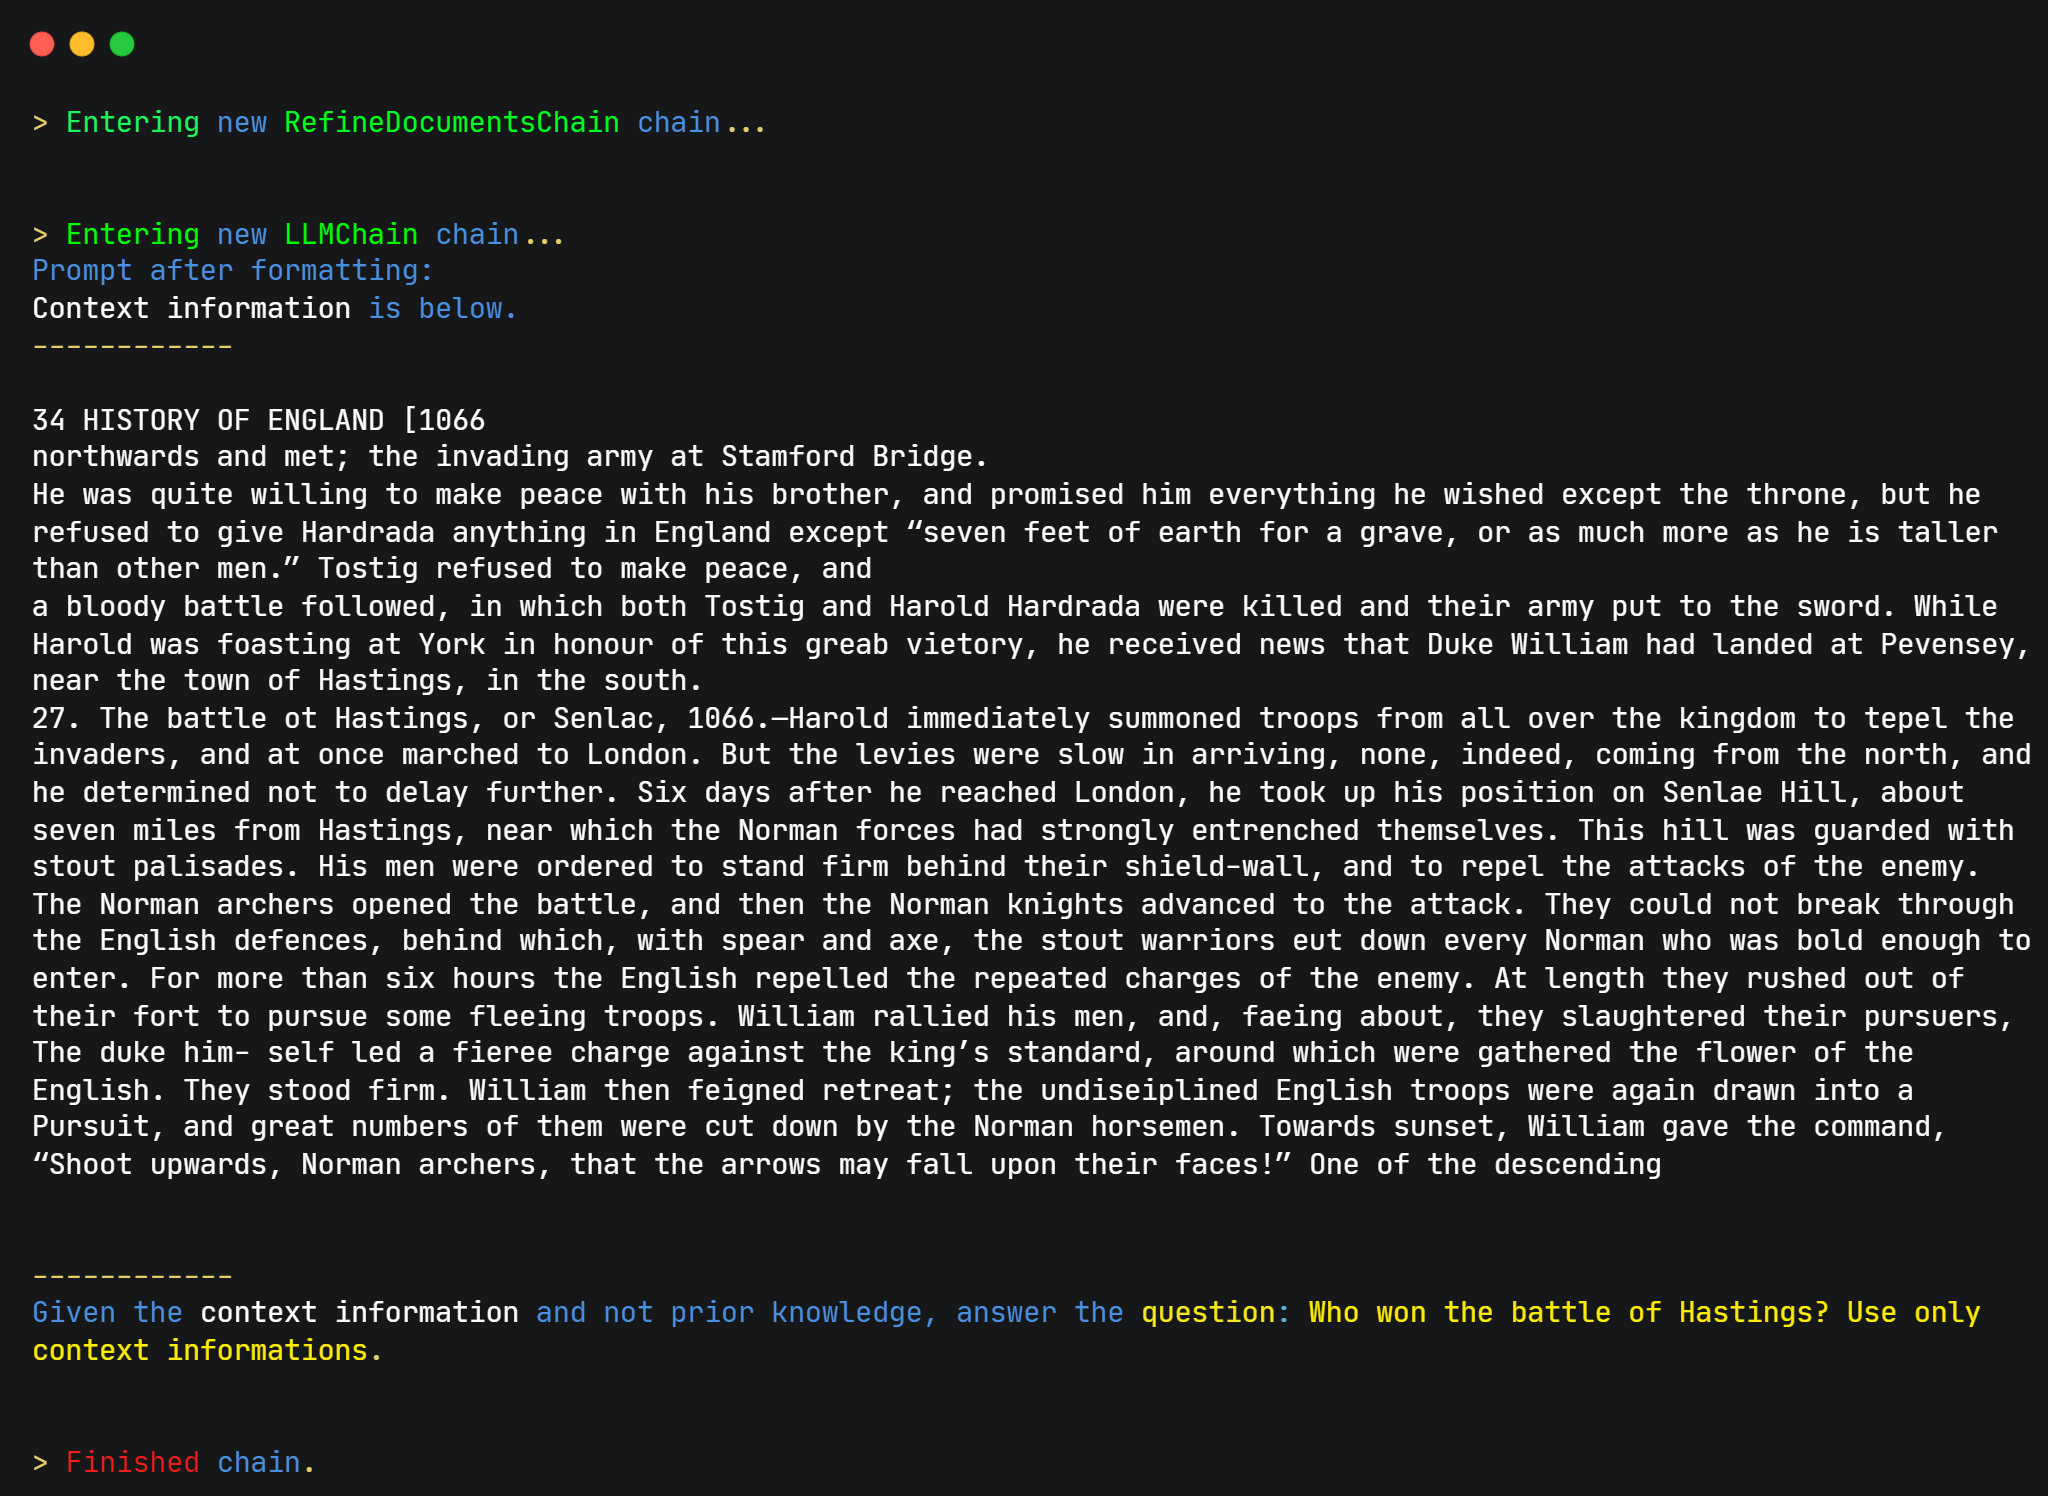
\includegraphics[width=0.7\pdfpagewidth]{images/refine_step_1.png}
\end{figure}
Questo è il primo passaggio dell'algoritmo di Refine e il primo documento viene inserito all'interno della input per intero, sono presenti inoltre alcune informazioni che LangChain inserisce per istruire il modello a non fare più di ciò che gli si sta chiedendo, questo è un problema comune sopratutto quando si modifica un parametro particolare degli LLM che viene definito "temperatura" ed indica quanto il modello debba utilizzare la sua parte creativa per dare la risposta.


\begin{figure}[H]
    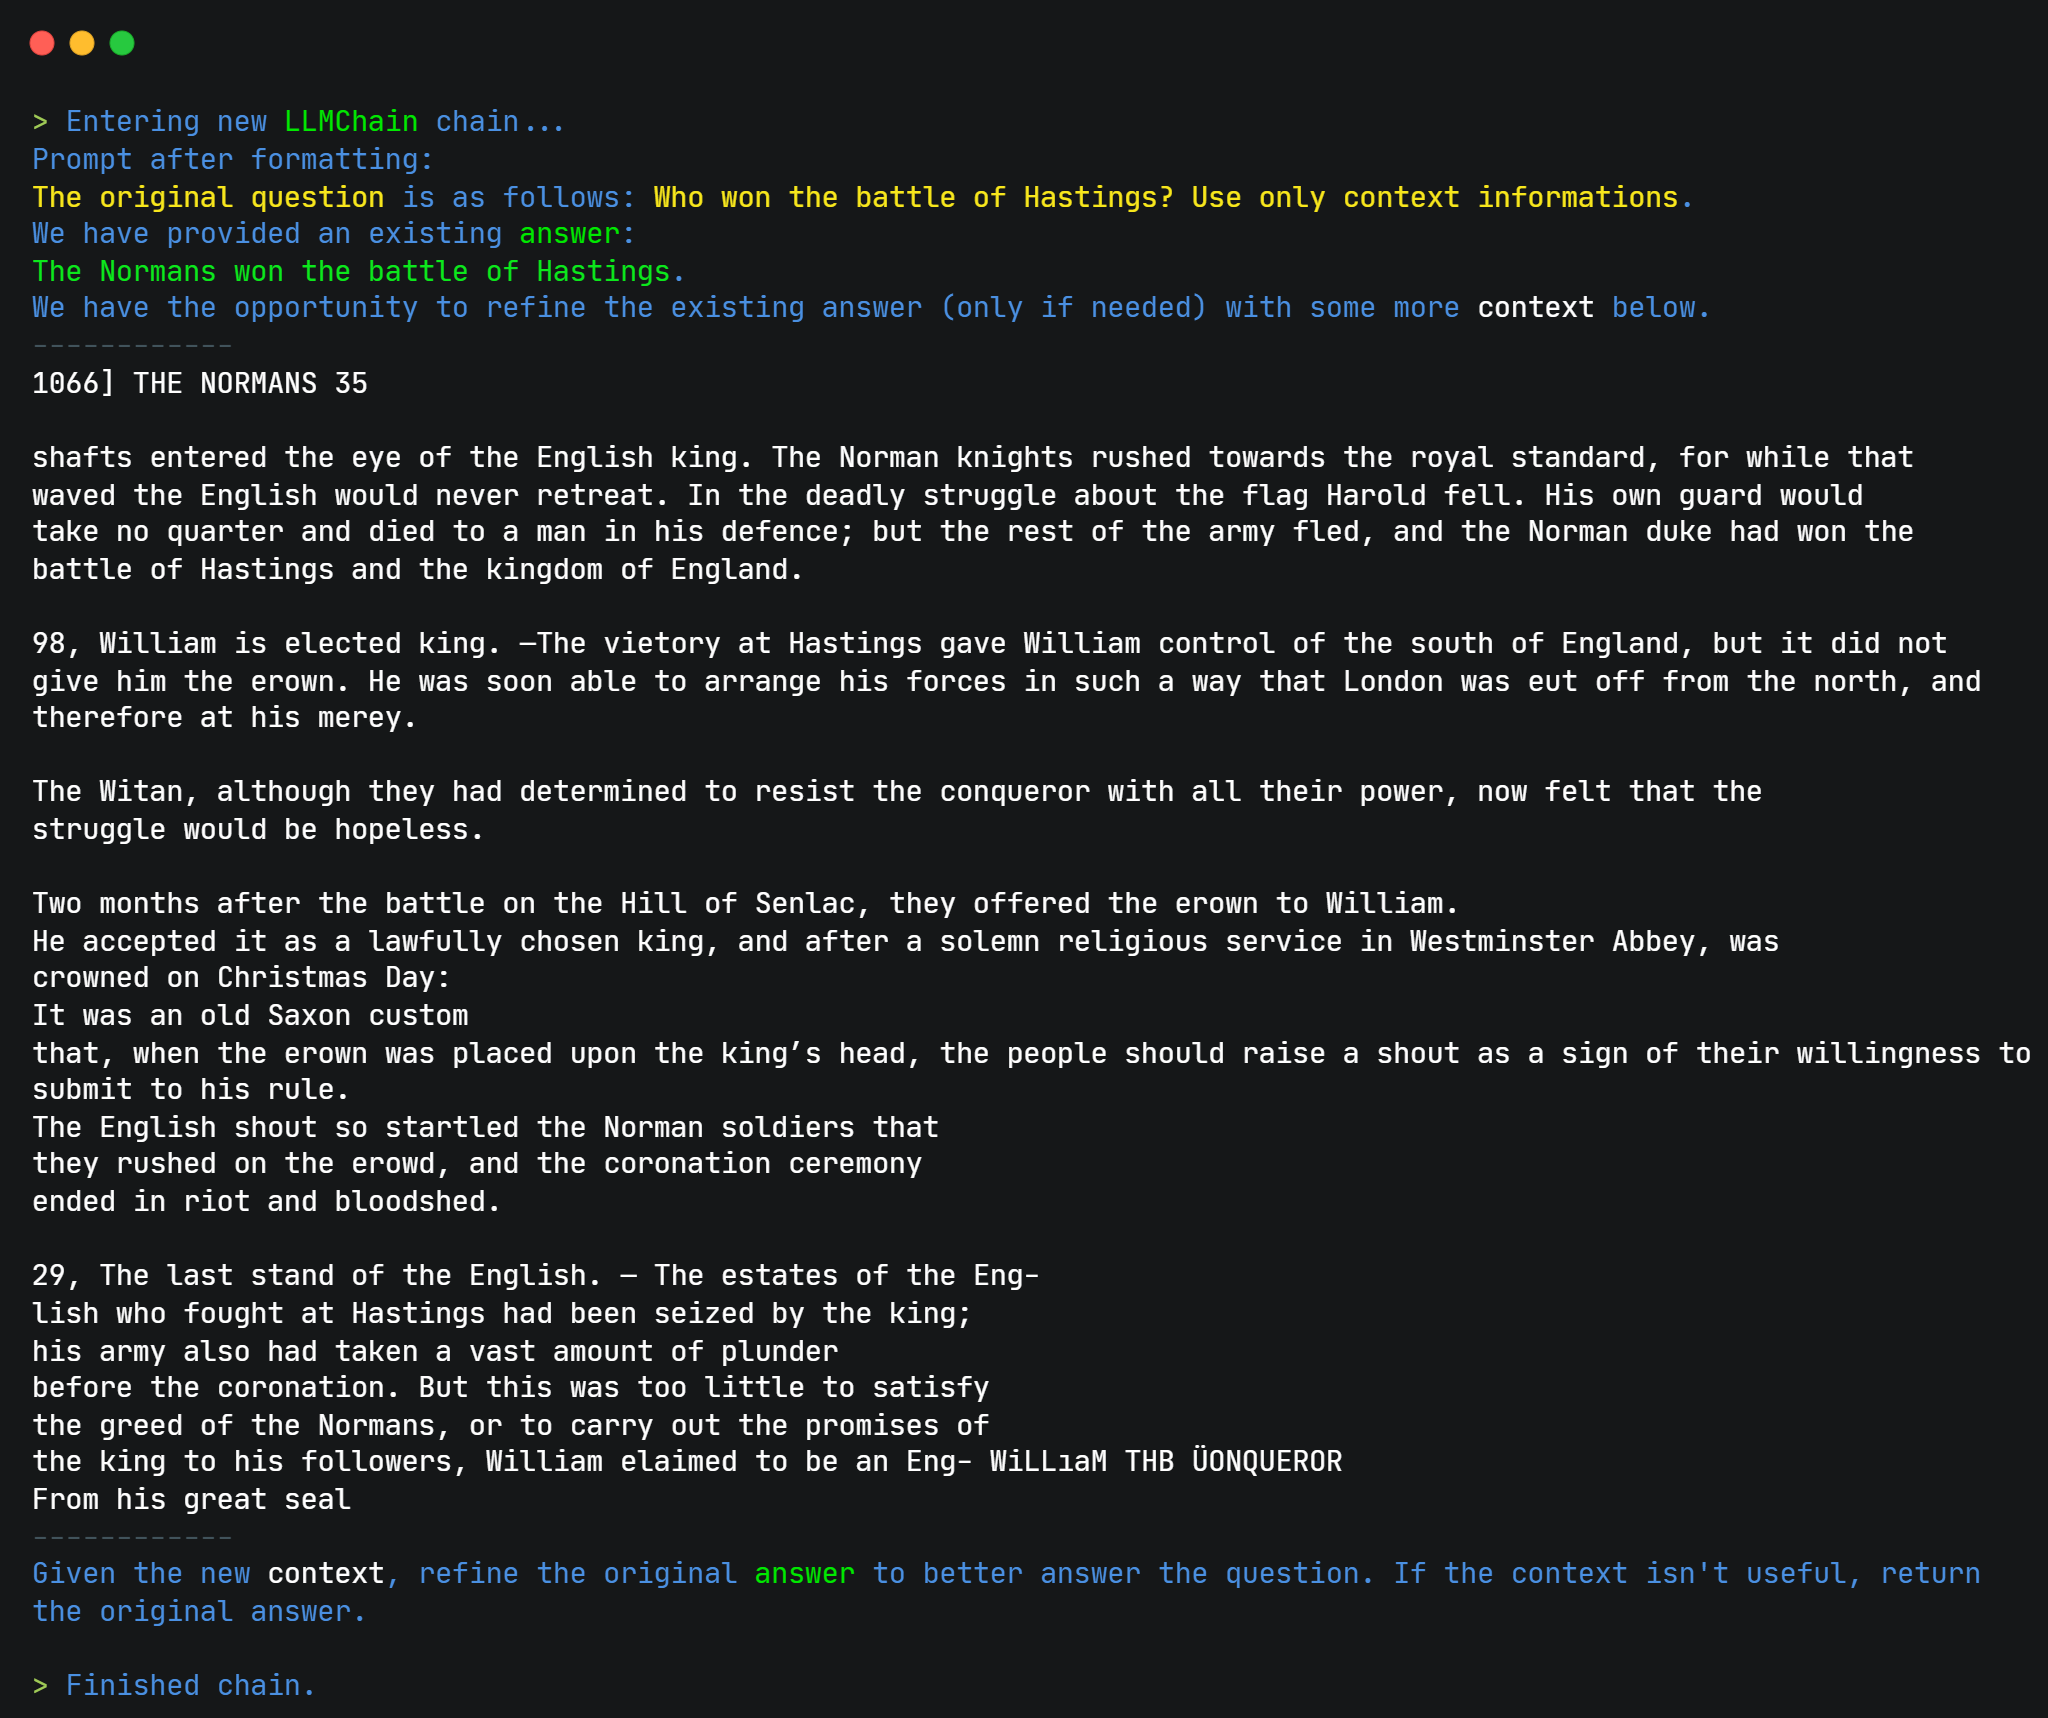
\includegraphics[width=0.7\pdfpagewidth]{images/refine_step_2.png}
\end{figure}

Questo è invece come avviene il processo di refine.
È possibile osservare come l'input iniziale al sistema viene cambiato aggiungendogli la prima risposta che il sistema è riuscito a trarre ``The Normans won the battle of Hastings'' e viene detto al modello che abbiamo la possibilità di migliorare la risposta con il contesto aggiuntivo dato dall'n-esimo documento (in questo caso il secondo). Questo passaggio viene effettuato per tutti i documenti che il SelfQueryRetriever ha trovato.
\newpage
Alla fine ciò che si ottiene è la risposta finale, che in questo caso è:

\begin{figure}[H]
    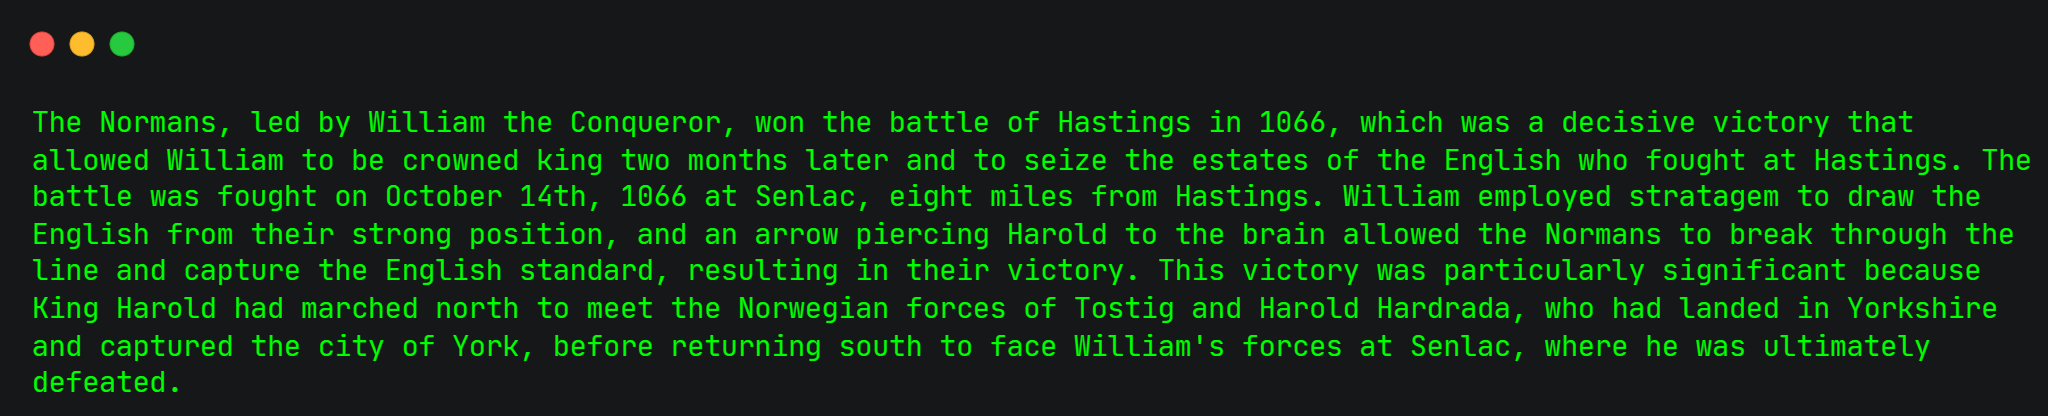
\includegraphics[width=0.7\pdfpagewidth]{images/refine_step_3.png}
\end{figure}

\subsection{I documenti presi in considerazione}
Per ogni query e risultato è possibile ottenere la lista dei chunk presi in considerazione dal sistema, per rispondere a questa domanda i chunk appartenevano a due libri diversi PPN1736870556.pdf, il cui titolo è ``Egland's story'' del 1918 e PPN1736868691.pdf, il cui titolo è ``Outlines of British history'' del 1885. Il frontespizio di entrambi i libri è visibile nella figura ~\ref{fig:libri}.
Oltre al semplice nome viene restituita anche la pagina del libro nella quale quel chunk era contenuto oltre a tutti i metadati inseriti in fase di ingestion.
\begin{figure}[H]
    
\includegraphics[width=0.5\textwidth]{images/engstory.png}
    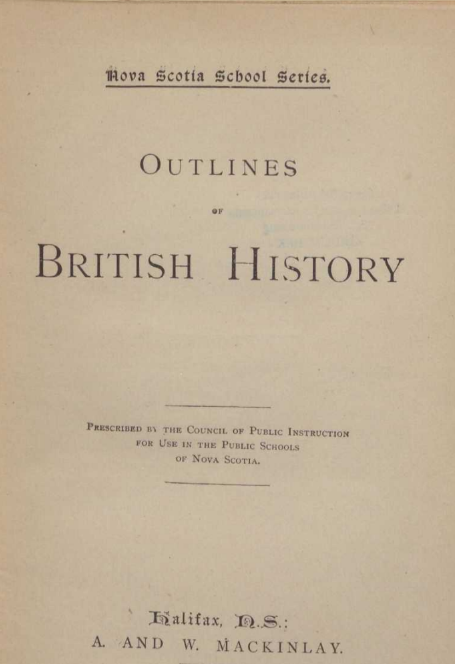
\includegraphics[width=0.5\textwidth]{images/b_history.png}
    \caption{Il frontespizio dei due libri presi in considerazione per la query ``Who won the battle of Hastings?''}
    \label{fig:libri}
\end{figure}